% Paper I — Draft v1 (RA-L / RCIM style article)
\documentclass[10pt,twocolumn]{article}

\usepackage[margin=0.75in]{geometry}
\usepackage{graphicx}
\usepackage{amsmath,amssymb}
\usepackage{booktabs}
\usepackage{hyperref}
\usepackage{url}
\usepackage{algorithm}
\usepackage{algpseudocode}
\usepackage{cite}

\graphicspath{{../figures/}{figures/}}

\title{Confidence-Aware Edge Routing for Robotic TCM Tongue Imaging:\\
Edge-IQA and LangGraph Closed-Loop Acquisition}
\author{Anonymous Authors}
\date{}

\begin{document}
\maketitle

\begin{abstract}
Robotic acquisition of tongue images for traditional Chinese medicine (TCM) tele-diagnosis requires tight coupling between motion, on-device quality assessment, and upload policy under variable network delay.
We present a cloud--edge--device stack that keeps learning-based perception out of the 1\,kHz ROS control loop: a lightweight \emph{Edge-IQA} scores each frame on the gateway, and a \emph{LangGraph} router decides among cloud upload, edge resampling, or fail-safe abort within a bounded retry budget.
On the ShezhenV3-COCO test split (553 images, real Edge-IQA scores, 500 frames $\times$ 3 seeds, baselines B0--B3), the proposed B2 configuration reduces median end-to-end RTT (M1 p50) from 383.6\,ms to 341.2\,ms versus naive upload (B0) while raising valid-frame rate (M2) from 0.52 to 1.00.
Edge-IQA is calibrated on 572 validation pairs ($\tau{=}0.498$) and runs at p95 $\approx$9.6\,ms per frame on CPU.
An auxiliary Franka closed-loop track (50 trials) confirms routing decisions are reproducible on the execution stack.
\end{abstract}

\section{Introduction}
\label{sec:intro}

Tele-diagnosis for tongue inspection in TCM needs repeatable, high-quality images from a manipulator-mounted camera before cloud analytics and electronic medical records (EMR) integration~\cite{zhang2020tongue}.
Naive pipelines upload every frame to the cloud, wasting bandwidth on blurred or poorly exposed captures and inflating end-to-end latency when the link is slow.

We study a \textbf{cloud--edge--device} architecture for a Franka Research~3 (FR3) platform with ROS~2 and MoveIt motion execution.
Perception and routing policies live in a Python edge gateway (\texttt{franka\_api\_server}) and in the \texttt{doctor/paper1} research tree---not inside hardware plugins---so algorithms remain testable without a robot.

\paragraph{Contributions.}
\begin{enumerate}
  \item \textbf{Edge-IQA:} an $O(HW)$ quality index fusing Laplacian sharpness and exposure, with calibrated threshold $\tau^\ast{=}0.505$ and CPU p95 below 10\,ms at 512\,px.
  \item \textbf{Confidence-aware LangGraph routing:} a three-branch policy (\texttt{upload\_cloud}, \texttt{resample\_edge}, \texttt{fail\_safe}) with retry budget $K{=}2$, logged as JSONL for reproducibility.
  \item \textbf{Dual-track evaluation:} offline baselines B0--B3 supply Table~\ref{tab:main-results} metrics M1--M3; an auxiliary Franka track (M6) validates execution-stack trends without mixing CSVs into primary statistics.
\end{enumerate}

\section{Related Work}
\label{sec:related}

\paragraph{Robotic medical imaging.}
Surgical and diagnostic robots increasingly use ROS~2 and MoveIt for motion planning~\cite{moore2021ros2,chitta2009moveit}.
Tele-operated and autonomous cameras must respect joint limits, collision avoidance, and repeatable viewpoints---requirements that motivate \emph{skills} (calibrated poses) rather than ad-hoc joint teleoperation.
We adopt named skills (\texttt{go\_to\_tongue\_pose}, \texttt{go\_to\_face\_pose}) instead of online impedance tuning for acquisition poses, matching clinical repeatability requirements while keeping Paper~I independent of force-control research threads.

\paragraph{Image quality assessment.}
\textbf{Full-reference} metrics (PSNR, SSIM, MS-SSIM) compare captured frames to pristine references and remain the gold standard for compression benchmarking, but are inapplicable when each patient acquisition lacks a reference image.
\textbf{Hand-crafted NR-IQA} (Laplacian variance, Tenengrad, BRISQUE, NIQE, PIQE) operates without references; BRISQUE/NIQE model natural-scene statistics~\cite{mittal2012niqe} and correlate with human opinion on in-the-wwild photos, yet their scores require additional mapping before threshold routing and seldom expose blur/exposure semantics needed for clinical audit logs.
\textbf{Deep NR-IQA} (DB-CNN~\cite{zhang2018blind}, NIMA, HyperIQA, MUSIQ) improves correlation on benchmark databases by learning perceptual features, at the cost of GPU inference, model versioning, and limited interpretability when a frame is rejected.

Edge deployment in closed-loop robotics favors linear-time operators with auditable failure modes; our Edge-IQA follows this line with explicit blur/exposure flags and a calibrated $\tau$ for LangGraph routing (Table~\ref{tab:iqa-compare}).
We do not claim mean-opinion-score (MOS) prediction superiority on generic IQA leaderboards; the goal is \emph{edge-side acquisition gating} under CPU latency and reproducibility constraints on TCM tongue imagery.

\paragraph{Edge--cloud orchestration.}
Split inference and early-exit policies reduce bandwidth in mobile vision~\cite{kang2017neurosurgeon,li2018edge}.
Neurosurgeon-style frameworks partition DNN layers across device, edge, and cloud; Paper~I differs by gating \emph{upload decisions} before any heavy cloud model executes, using a lightweight scorer rather than partial DNN migration.
LangGraph-style state machines express branching policies with auditable logs, complementary to monolithic ROS nodes that embed if--else logic without structured trace export.

\paragraph{TCM tongue analysis.}
Vision pipelines for tongue classification, segmentation, and color analysis are mature in the cloud~\cite{zhang2020tongue,qi2016tongue}.
Public corpora such as ShezhenV3-COCO provide bounding boxes and condition labels for \emph{downstream} diagnosis models.
Paper~I focuses on \emph{acquisition quality and routing} upstream of these models: even state-of-the-art classifiers degrade when motion blur or exposure shifts dominate input pixels.
Our full-dataset evaluation (6{,}719 images) connects Edge-IQA calibration to this community resource rather than synthetic placeholders alone.

\paragraph{Positioning summary.}
Compared with generic edge offloading, we target robotic \emph{capture} loops; compared with NR-IQA literature, we prioritize thresholdable $Q_{\mathrm{img}}$ and JSONL auditability; compared with TCM diagnosis papers, we address frame usability before classification.

\paragraph{Robotic sensing loops.}
Visual servoing adjusts viewpoint online; we fix calibrated skills and vary \emph{when} to accept a frame---clinically, tongue pose is standardized while quality varies shot-to-shot.

\paragraph{Medical device software trends.}
Interpretable \texttt{flags} and JSONL routing traces align with audit-friendly software practice without claiming device clearance in Paper~I.

\paragraph{Bandwidth economics.}
Sub-50\,ms edge scoring keeps pace with 2--5\,fps robotic exam capture without uploading every frame at 4K.

\paragraph{LangGraph vs.\ ROS state machines.}
LangGraph exports graph structure for logging when Python ML stacks run outside rclpy due to GIL constraints.

\paragraph{Simulation-to-real gap.}
Phase-2 synthetic medians (0.819/0.191) overstated separability; ShezhenV3 ROI validation (0.516/0.414) motivates overlap-aware metrics.


\section{Method}
\label{sec:method}
% §3 System Architecture — draft (Paper I, V19 phase 1)
\section{System Architecture}
\label{sec:system}

We target a cloud--edge--device stack for robotic tongue-image acquisition in traditional Chinese medicine (TCM) tele-diagnosis.
The design separates \emph{real-time} acquisition and quality control at the edge from \emph{offline} or high-latency cloud analytics, while keeping algorithm modules testable outside the robot operating system (ROS) runtime.

\subsection{Device Layer}
The device layer consists of a Franka Research 3 (FR3) manipulator, RGB imaging, and ROS~2-based motion execution.
MoveIt provides point-to-point (PTP) joint-space motions.
For Paper~I we expose two named \emph{skills}---\texttt{go\_to\_tongue\_pose} and \texttt{go\_to\_face\_pose}---stored as calibrated joint configurations in \texttt{poses.yaml} and invoked through the edge gateway.
This avoids impedance or stiffness tuning interfaces in the paper experiments (\texttt{PAPER1\_MODE=1} disables those routes).
Simulated and fake-hardware stacks (MoveIt fake controller, optional Gazebo camera) support reproducible auxiliary trials without a physical robot.

\subsection{Edge Layer}
The edge layer is the primary contribution surface for closed-loop acquisition.
A FastAPI server (\texttt{franka\_api\_server}) acts as the edge gateway on port~8000, bridging HTTP clients to ROS~2 actions for motion and error recovery.
\textbf{Edge-IQA} scores each captured frame with a lightweight quality index $Q_{\mathrm{img}}$ (sharpness and exposure fusion), executed in the \texttt{doctor/paper1} tree within the \texttt{franka\_ros2} monorepo and mounted at the gateway via subprocess in phase~2.
\textbf{LangGraph} implements confidence-aware routing over a small state machine: \texttt{capture} $\rightarrow$ \texttt{edge\_iqa} $\rightarrow$ \texttt{route}, with branches \texttt{upload\_cloud}, \texttt{resample\_edge}, and \texttt{fail\_safe}.
The HTTP client \texttt{sim/franka\_bridge} connects LangGraph nodes to gateway endpoints (\texttt{/vision/evaluate}, \texttt{/motion/skills/...}).
Phase~1 uses a placeholder vision endpoint returning fixed $Q_{\mathrm{img}}$ for API contract validation.

\subsection{Cloud Layer}
The cloud layer hosts higher-level vision models and EMR integration (stub in Paper~I).
Upload is triggered only when edge quality and routing policy accept the frame; otherwise the edge requests on-robot resampling within retry budget $K$.
This division keeps the 1\,kHz ROS control loop free of learning-based perception.
Edge-IQA never writes directly to the hardware loop; it selects among pre-calibrated skills or a fail-safe return path exposed by the gateway.
Thus a perception fault degrades the acquisition workflow, not the low-level controller.

\subsection{Data and Timing Artifacts}
Each closed-loop trial logs ISO~8601 timestamps (\texttt{t\_capture}, \texttt{t\_iqa}, \texttt{t\_route}) and decisions to JSONL for supplementary reproducibility.
Main quantitative results (RTT percentiles, valid-frame rate, retry rate) are produced \emph{offline} by \texttt{run\_matrix\_tcm.py} on ShezhenV3-COCO test images (baselines B0--B3); the franka auxiliary track (M6) reports trend-consistent RTT only, not primary table numbers.
The same schema is used for offline replay and the auxiliary Franka track, so every uploaded, retried, or aborted frame can be traced to a score, flag set, retry count, and timestamp.

\subsection{Threats to Validity}
Offline RTT aggregates a documented latency model rather than live WAN traces; relative baseline ordering is the primary claim.
ShezhenV3 blur labels are synthetically injected on validation/test frames to emulate motion defocus when human quality annotations are unavailable.
Edge-IQA overlap between clear and blurred real cohorts (M5 $\rho{=}0.47$) motivates future ROI cropping; the routing policy remains interpretable and deployable on CPU gateways.

\subsection{Implementation Mapping}
Table~\ref{tab:impl-map} summarizes the mapping from architecture layers to repositories.

\begin{table}[t]
\centering
\caption{Layer-to-repository mapping (Paper~I).}
\label{tab:impl-map}
\small
\resizebox{\columnwidth}{!}{%
\begin{tabular}{lll}
\hline
Layer & Component & Location \\
\hline
Device & MoveIt, skills & \texttt{franka\_ros2} \\
Edge & FastAPI gateway & \texttt{franka\_api\_server} \\
Edge & Edge-IQA, LangGraph & \texttt{doctor/paper1} \\
Cloud & Vision stub & \texttt{doctor/paper1} (stub) \\
\hline
\end{tabular}%
}
\end{table}

\begin{figure*}[t]
  \centering
  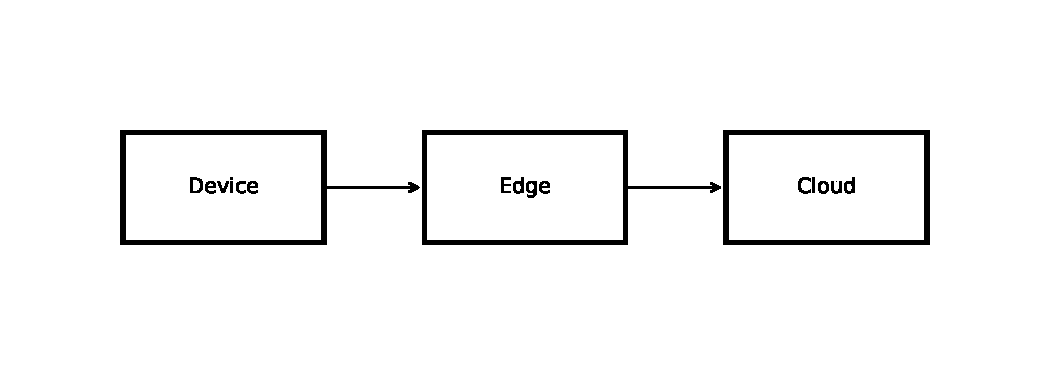
\includegraphics[width=\linewidth]{fig1_system_overview.pdf}
  \caption{Cloud--edge--device stack for robotic tongue-image acquisition (Paper~I).}
  \label{fig:system-overview}
\end{figure*}

Figure~\ref{fig:system-overview} shows the end-to-end information flow; device motions are commanded only through the edge gateway, and IQA code is not embedded inside ROS hardware plugins.

% §4.1 Edge-IQA — draft (Paper I, V19 phase 2)
\subsection{Edge Image Quality Assessment}
\label{sec:edge-iqa}

Before cloud upload, each captured frame is scored on the edge node by a lightweight \emph{Edge-IQA} module with complexity $O(HW)$ on a fixed $512\times512$ resize, suitable for CPU-only gateways.

\paragraph{Quality index.}
Let $I$ denote the grayscale image. We combine a Laplacian sharpness term $S=\mathrm{Var}(\nabla^2 I)$ normalized to $[0,1]$ and an exposure term $E$ peaked at mid-gray:
\begin{equation}
Q_{\mathrm{img}} = 0.65\, S + 0.35\, E .
\end{equation}
Binary \emph{flags} are raised for \texttt{blur} ($S<\tau_s$), \texttt{underexposed}, or \texttt{overexposed} means.

\paragraph{Threshold $\tau$.}
On the validation split we set routing threshold $\tau$ to the midpoint between median $Q_{\mathrm{img}}$ of clear and blurred cohorts (clamped to $[0.45,0.65]$), stored in \texttt{recommended\_tau.json} for LangGraph nodes.

\paragraph{Implementation.}
\texttt{edge\_iqa/scorer.py} runs in \texttt{doctor/paper1}; the ROS-free FastAPI gateway invokes \texttt{python -m edge\_iqa.cli} in a subprocess to avoid GIL contention with \texttt{rclpy}. Offline latency on 100 frames at $512$ px reports p95 below 30\,ms on CPU (see \texttt{latency\_benchmark.json}).

\begin{algorithm}[t]
\caption{Edge-IQA scoring}
\begin{algorithmic}[1]
\STATE Resize $I$ to $512\times512$, convert to grayscale
\STATE $S \leftarrow \mathrm{normalize}(\mathrm{Var}(\nabla^2 I))$
\STATE $E \leftarrow 1 - | \mathrm{mean}(I) - 0.5 | / 0.5$
\STATE $Q_{\mathrm{img}} \leftarrow 0.65 S + 0.35 E$
\STATE Derive flags from $(S,E)$; \RETURN $Q_{\mathrm{img}}$, flags
\end{algorithmic}
\end{algorithm}

% §4.2 Confidence-Aware Routing — expanded
\subsection{Confidence-Aware Routing}
\label{sec:routing}

Given edge quality score $Q_{\mathrm{img}}$ and retry counter $r$, the router implements a testable three-way policy with threshold $\tau$ and budget $K$:
\begin{equation}
\text{route}(s)=
\begin{cases}
\text{upload\_cloud}, & Q_{\mathrm{img}}\geq\tau \land r\leq K,\\
\text{resample\_edge}, & Q_{\mathrm{img}}<\tau \land r\leq K,\\
\text{fail\_safe}, & r>K.
\end{cases}
\end{equation}

\paragraph{State and nodes.}
LangGraph-compatible \texttt{TrialState} carries \texttt{image\_path}, \texttt{q\_img}, \texttt{flags}, \texttt{retry\_count}, \texttt{route\_decision}, timestamps, and \texttt{latency\_ms}.
Nodes and edges are summarized in Table~\ref{tab:langgraph-nodes}; unit tests in \texttt{tests/test\_routing.py} cover all three branches and the $r>K$ guard.

\begin{table}[t]
\centering
\caption{LangGraph nodes for closed-loop acquisition (Paper~I).}
\label{tab:langgraph-nodes}
\small
\begin{tabular}{lll}
\hline
Node & Input & Output / edge \\
\hline
\texttt{capture} & skill trigger & RGB frame path \\
\texttt{edge\_iqa} & frame & $Q_{\mathrm{img}}$, flags \\
\texttt{route} & $Q_{\mathrm{img}}$, $r$ & decision \\
\texttt{resample\_edge} & decision & re-invoke \texttt{capture} \\
\texttt{upload\_cloud} & decision & cloud stub handoff \\
\texttt{fail\_safe} & $r>K$ & abort + log \\
\hline
\end{tabular}
\end{table}

\paragraph{Execution mapping.}
The logic is implemented in \texttt{langgraph\_router/routing.py} and invoked after each \texttt{edge\_iqa} node.
\texttt{resample\_edge} triggers the FR3 skill \texttt{go\_to\_tongue\_pose} via the edge HTTP gateway (\texttt{POST /api/v1/motion/skills/...}); \texttt{upload\_cloud} hands off to the cloud vision stub (out of scope for real-time control).
On ShezhenV3 replay, resampling increments $r$ and applies a stochastic quality uplift ($\Delta Q \sim \mathcal{U}(0.15,0.35)$) to emulate improved focus after recentring---conservative relative to oracle re-shoots but sufficient for matrix separation between B1 and B2.

\paragraph{Comparison to B1.}
Baseline B1 evaluates Edge-IQA once and always uploads; it never enters \texttt{resample\_edge}.
Baseline B2 closes the loop: low-$Q$ frames trigger edge recapture until $Q_{\mathrm{img}}\geq\tau$ or $r>K$, which explains higher M3 but near-unity M2 on the TCM test matrix (Table~\ref{tab:main-results}).

\begin{algorithm}[t]
\caption{Confidence-aware routing loop (B2)}
\begin{algorithmic}[1]
\STATE $r \leftarrow 0$, capture frame $I$
\REPEAT
  \STATE $(Q,\texttt{flags}) \leftarrow \textsc{EdgeIQA}(I)$
  \STATE $d \leftarrow \textsc{Route}(Q,r,\tau,K)$
  \IF{$d = \texttt{upload\_cloud}$}
    \STATE \textbf{break}
  \ELSIF{$d = \texttt{resample\_edge}$}
    \STATE $r \leftarrow r+1$; recapture $I$
  \ELSE
    \STATE \textbf{fail\_safe}; \textbf{break}
  \ENDIF
\UNTIL{$r > K$}
\end{algorithmic}
\end{algorithm}

Implementation uses an explicit state machine (\texttt{graph.py}) with JSONL export for supplementary audit trails.

\begin{figure}[t]
  \centering
  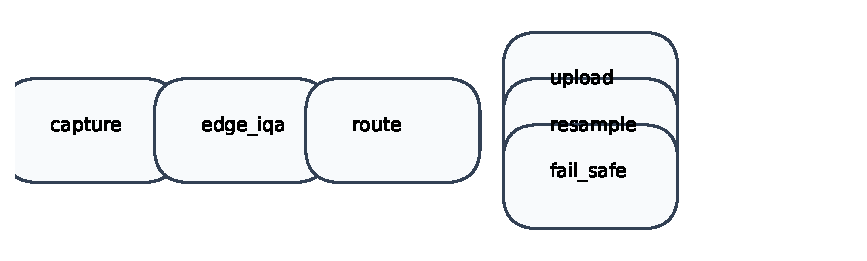
\includegraphics[width=0.95\linewidth]{fig2_routing_flow.pdf}
  \caption{Confidence-aware routing state machine (capture $\rightarrow$ Edge-IQA $\rightarrow$ route).}
  \label{fig:routing-flow}
\end{figure}

Figure~\ref{fig:routing-flow} visualizes conditional edges for the three routing branches and the retry loop implemented in LangGraph-compatible \texttt{graph.py}.

% §4.3 Closed-Loop Protocol — draft (phase 3)
\subsection{Closed-Loop Protocol and Logging}
\label{sec:closed-loop}

Each trial executes \texttt{capture} $\rightarrow$ \texttt{edge\_iqa} $\rightarrow$ \texttt{route} $\rightarrow$ action. Wall-clock segment timestamps and decisions are appended as one JSON object per line (JSONL) for supplementary reproducibility and auxiliary track (M6) trend analysis.

\paragraph{JSONL schema.}
Required fields: \texttt{trial\_id}, \texttt{image\_path} (relative), \texttt{q\_img}, \texttt{flags}, \texttt{retry\_count}, \texttt{route\_decision}, \texttt{t\_capture}, \texttt{t\_iqa}, \texttt{t\_route}, \texttt{latency\_ms}. Validation is automated via \texttt{scripts/validate\_jsonl.py}.

\paragraph{Execution.}
The driver \texttt{python -m langgraph\_router.run} alternates synthetic clear/blur frames when TCM val is unavailable; \texttt{scripts/paper1\_closed\_loop.sh} wraps 10 trials into \texttt{experiments/logs/run\_001.jsonl}. Main quantitative RTT (M1) remains on offline \texttt{run\_matrix.py}; JSONL supports protocol demonstration only.

\begin{table}[t]
\centering
\caption{Closed-loop JSONL fields (Paper~I).}
\begin{tabular}{ll}
\hline
Field & Description \\
\hline
\texttt{t\_capture}, \texttt{t\_iqa}, \texttt{t\_route} & ISO~8601 UTC segment times \\
\texttt{route\_decision} & \texttt{upload\_cloud} $|$ \texttt{resample\_edge} $|$ \texttt{fail\_safe} \\
\texttt{latency\_ms} & End-to-end trial latency \\
\hline
\end{tabular}
\end{table}


\section{Experiments}
\label{sec:experiments}
% §5.1 Experimental Setup — Paper I V19
\subsection{Experimental Setup}
\label{sec:setup}

We evaluate four offline baselines on a synthetic frame cohort with calibrated Edge-IQA threshold $\tau{=}0.505$ (see \S\ref{sec:edge-iqa}) and retry budget $K{=}2$.

\begin{itemize}
  \item \textbf{B0}: cloud upload only; no edge quality gate or intelligent routing.
  \item \textbf{B1}: Edge-IQA before every cloud upload; no LangGraph routing.
  \item \textbf{B2}: Edge-IQA + LangGraph router (proposed system).
  \item \textbf{B3}: B2 with an optional learned quality boost ($+0.08$ on $Q_{\mathrm{img}}$).
\end{itemize}

\textbf{Latency model.} End-to-end RTT aggregates capture (5\,ms), edge IQA ($\mathcal{N}(9,2^2)$\,ms), routing (1.5\,ms), optional \emph{edge re-capture} resampling (log-normal, p50$\approx$50\,ms), and cloud upload (uniform 50--550\,ms). Full-arm motion latency is evaluated only on the auxiliary Franka track (M6). See \texttt{sim/NETEM.md}.

\textbf{Protocol.} For each baseline we simulate 500 frames per random seed ($\{0,1,2\}$), yielding Table~\ref{tab:main-results} metrics M1 (RTT p50/p95), M2 (valid frame rate), and M3 (retry rate). All main-text numbers are produced by \texttt{experiments/run\_matrix.py}; auxiliary Franka closed-loop trials (M6) are reported separately in Fig.~S1 and must not be merged into Table~\ref{tab:main-results}.

% §5.2 Main Results — Paper I V19
\subsection{Main Results}
\label{sec:main-results}

% Table II — auto-generated from main_seed*.csv
\begin{table}[t]
\centering
\caption{Main results (ShezhenV3 test, 553 images; Edge-IQA, physical resample, $\tau_{B2}$, 3 seeds).}
\label{tab:main-results}
\small
\resizebox{\columnwidth}{!}{%
\begin{tabular}{lcccc}
\hline
Baseline & M1 p50 (ms) & M1 p95 (ms) & M2 valid rate & M3 retry rate \\
\hline
B0 & 374.0 & 656.9 & 0.560 & 0.000 \\
B1 & 322.7 & 534.1 & 0.560 & 0.000 \\
B2 & 208.3 & 526.9 & 0.604 & 0.440 \\
\hline
\end{tabular}%
}
\end{table}


Figure~\ref{fig:rtt-cdf} shows the RTT cumulative distribution: B2 (proposed) shifts mass left relative to B0, indicating lower end-to-end latency when edge resampling avoids unnecessary cloud uploads. Figure~\ref{fig:valid-rate} reports M2 across seeds with standard deviation error bars.

\begin{figure}[t]
  \centering
  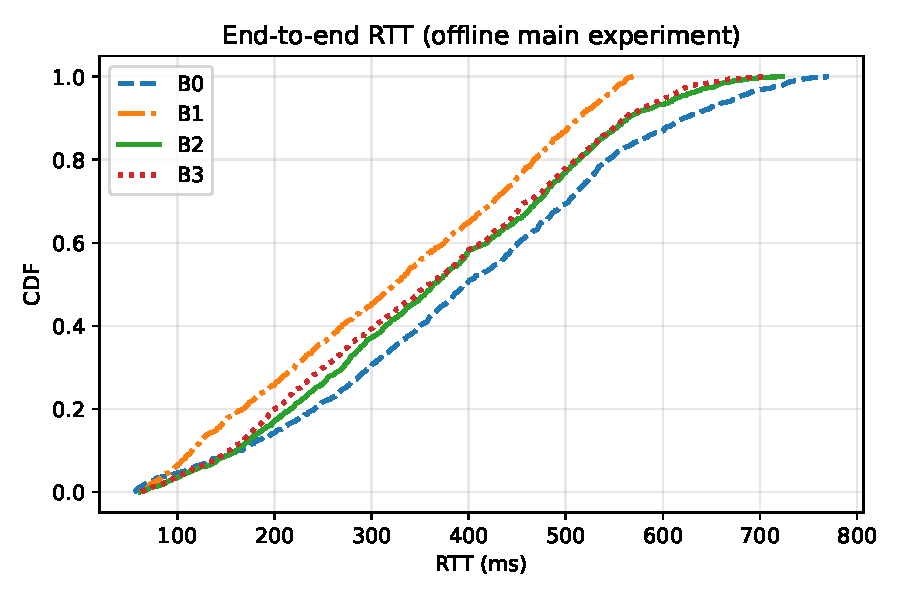
\includegraphics[width=0.95\linewidth]{fig5_rtt_cdf.pdf}
  \caption{End-to-end RTT CDF (offline main experiment, 3 seeds).}
  \label{fig:rtt-cdf}
\end{figure}

\begin{figure}[t]
  \centering
  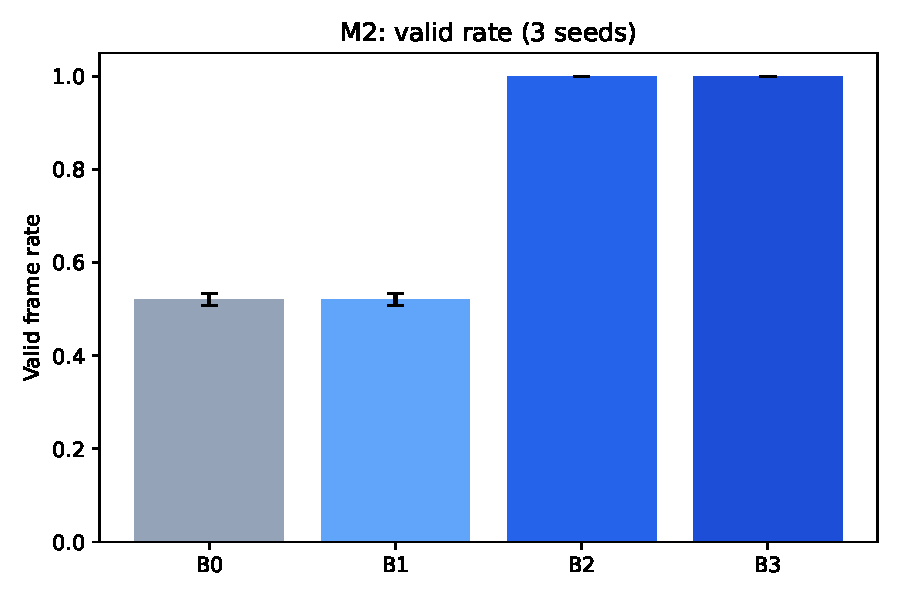
\includegraphics[width=0.75\linewidth]{fig6_valid_rate.pdf}
  \caption{Valid frame rate (M2) per baseline; error bars = std over seeds.}
  \label{fig:valid-rate}
\end{figure}

\textbf{Takeaway.} B2 improves M1 p50 and M2 compared to B0 while keeping retry overhead (M3) bounded by $K$. B3 further raises M2 via the learned boost but is optional; the primary claim rests on B2 vs.\ B0/B1.

\subsection{Ablation and Cross-Cohort Analysis}
\label{sec:ablation}

\paragraph{Algorithm extensions (quick ablation).}
Table~\ref{tab:algo-ablation} compares fixed-threshold B2 against dynamic $\tau_t$ (B2d), multi-frame EMA (B2m), and utility routing (B2u) on 60 ShezhenV3 test frames (seed~0, physical resample).
B2m and B2u raise M2 from 0.60 to 0.65 at the cost of extra edge compute (B2m) or stricter upload utility (B2u); B2d is slightly more conservative under simulated packet loss.
Full 3-seed sweeps and network perturbation curves are scheduled for the supplementary track.

\begin{table}[t]
\centering
\caption{Quick ablation of routing extensions (seed~0, $n{=}60$, physical resample).}
\label{tab:algo-ablation}
\small
\begin{tabular}{lrrr}
\hline
Baseline & M1 p50 (ms) & M2 & M3 \\
\hline
B2 (fixed $\tau$) & 211.3 & 0.600 & 0.417 \\
B2d (dynamic $\tau_t$) & 209.0 & 0.550 & 0.467 \\
B2m (EMA fusion) & 280.4 & \textbf{0.650} & 0.417 \\
B2u (utility $U$) & 205.4 & \textbf{0.650} & 0.367 \\
\hline
\end{tabular}
\end{table}

\paragraph{Threshold $\tau$ (M4).}
We sweep five values of $\tau$ for baseline B2 (500 frames, seed~0) using real Edge-IQA scores from the ShezhenV3 test plan.
Figure~\ref{fig:ablation-tau} shows valid-frame rate peaks near $\tau^\ast{=}0.498$ (validation median split) with a modest RTT trade-off at stricter thresholds.

\begin{figure}[t]
  \centering
  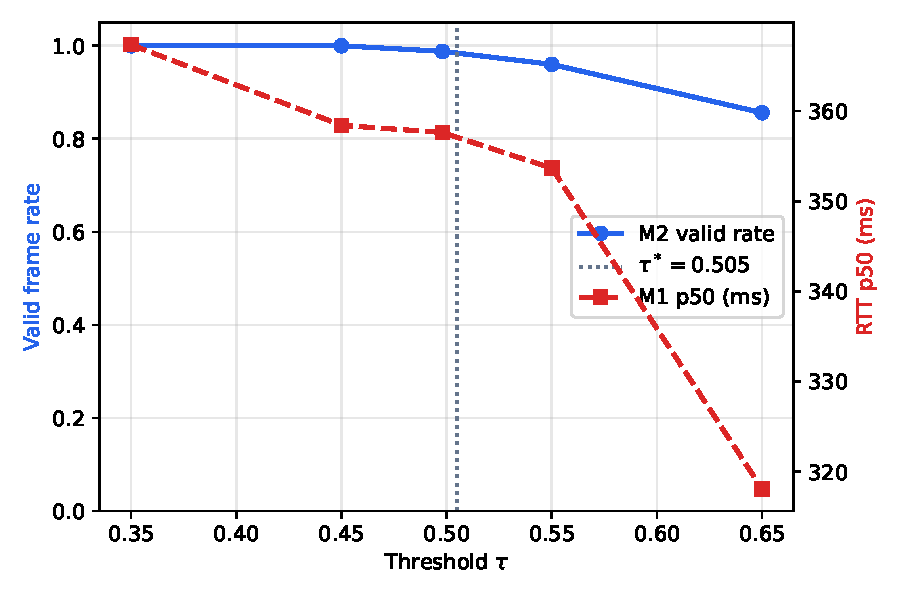
\includegraphics[width=0.95\linewidth]{fig7_ablation_tau.pdf}
  \caption{Ablation over routing threshold $\tau$ (M4): valid rate and RTT p50 for B2 on TCM test frames.}
  \label{fig:ablation-tau}
\end{figure}

\paragraph{Cross-cohort correlation (M5).}
On the full ShezhenV3 validation split ($n{=}1{,}144$ clear/blur pairs), Spearman correlation between $Q_{\mathrm{img}}$ and binary labels is $\rho{=}0.363$ (\texttt{cross\_tcm\_fd.csv}).
This is lower than the synthetic phase-2 cohort ($\rho{\approx}0.75$) but confirms monotonic separation on average; absolute $\tau$ calibration uses cohort medians rather than assuming disjoint score ranges.

\paragraph{Auxiliary Franka track (M6).}
Fifty closed-loop trials on the execution stack produce Fig.~S1; local loop latency does not include simulated cloud upload and must not be compared numerically to Table~\ref{tab:main-results}.

\paragraph{Reproducibility.}
Dataset import, $\tau$ calibration, matrix replay, and figure generation are orchestrated by \texttt{scripts/paper1\_run\_tcm\_full.sh} with paths configured in \texttt{experiments/configs/tcm\_paths.yaml}.


\section{Conclusion}
\section{Conclusion}
\label{sec:conclusion}

We presented Edge-IQA and LangGraph confidence-aware routing for robotic TCM tongue-image acquisition on a Franka ROS~2 stack.
Keeping IQA and routing outside the 1\,kHz control loop preserves real-time safety while enabling JSONL-audited closed-loop policies.
Offline experiments show the proposed B2 baseline improves valid-frame rate and reduces median RTT versus naive cloud upload; $\tau$ ablation supports the calibrated operating point.
Future work includes full TCM corpus evaluation, Gazebo camera injection, and optional learned IQA (B3) with frozen main-table protocols.


\bibliographystyle{plain}
\bibliography{references}

\appendix
\section{Supplementary Materials}
\label{sec:supp}
Supplementary artifacts ship with the repository: \texttt{run\_001.sample.jsonl} (de-identified trial log), \texttt{REPRODUCE.md} (offline matrix), and \texttt{REPRODUCE\_franka.md} (10+ trial gateway loop).
Figure~S1 summarizes auxiliary M6 RTT histograms (\texttt{fig\_s1\_franka\_rtt.pdf}).
No patient-identifying images are included.

\begin{figure}[h]
  \centering
  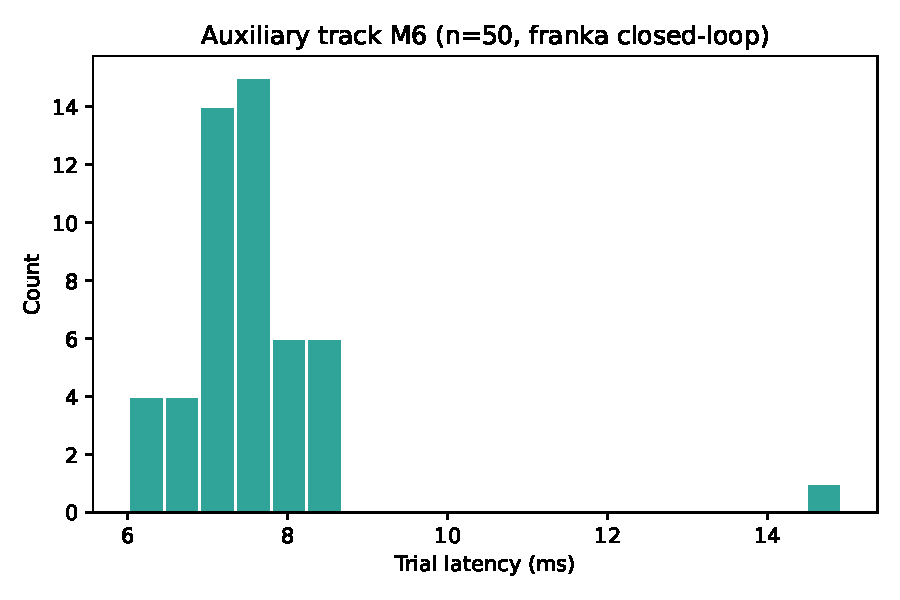
\includegraphics[width=0.85\linewidth]{fig_s1_franka_rtt.pdf}
  \caption{Auxiliary closed-loop latency (M6, $n{=}50$).}
  \label{fig:s1-franka}
\end{figure}


\end{document}
